\documentclass[12pt]{article}
\author{Rien Maertens\\
    2\textsuperscript{de} Bachelor Informatica}
    \title{Project Zeepbelbomen}
    \usepackage[utf8]{inputenc}
    \usepackage[dutch]{babel}
    \usepackage{amsthm}
    \usepackage{enumerate}
    \usepackage{mathtools}
    \usepackage{graphicx}
    \usepackage{tikz}
    \usepackage{pgfplots}
    \usepackage{pgfplotstable}
    \pgfplotsset{compat=1.10}
    \usetikzlibrary{shapes.geometric,arrows,fit,matrix,positioning}
    \tikzset
    {
    	tr/.style = {circle, draw=black, align=center, minimum size=1cm}
    }
    \DeclarePairedDelimiter\floor{\lfloor}{\rfloor} 

    \newtheorem{opgave}{Opgave}
    \newtheorem{geval}{Geval}[subsection]

    \begin{document}
    \maketitle
    \part*{Theoretische Vragen}
    \begin{opgave}
        Geen top in een bladzeepbel heeft een kind in een andere zeepbel.
        \begin{proof}
            Stel we hebben een bladzeepbel $\alpha$ met een top $T$ die een kind $K$ heeft in zeepbel $\beta$. 
            Neem $n$ het aantal zeepbellen dat het pad van zeepbel $\alpha$ naar de wortel bevat. 
            We kunnen de volgende twee gevallen onderscheiden:
            \begin{description}
                \item[Geval 1] Zeepbel $\beta$ bevat een top zonder kinderen en is dus een bladzeepbel.
                    Het pad van de wortel van de boom naar $\beta$ gaat door $\alpha$.
                    Dit pad bevat dus $n+1$ zeepbellen, wat in tegenstrijd is met het gegeven dat het pad van de wortel naar alle bladzeepbellen evenveel zeepbellen bevat.
                    Het gestelde is dus vals. Het is onmogelijk voor een bladzeepbel om een kind te hebben in een andere zeepbel.
                \item[Geval 2] Zeepbel $\beta$ is geen bladzeepbel, maar bevat wel een pad naar een top zonder kinderen.
                    Deze top is onderdeel van bladzeepbel $\gamma$.
                    Het pad van $\gamma$ naar de wortel van de zeepbelboom bevat $n+k$ zeepbellen, met $k$ het aantal zeepbellen in het pad tussen $\beta$ en $\gamma$.
                    Dit is opnieuw in tegenstrijd met het gegeven dat het pad van de wortel naar alle bladzeepbellen hetzelfde aantal zeepbellen bevat.
                    Ook in dit geval kan een bladzeepbel geen kinderen in andere zeepbellen hebben.
            \end{description}
        \end{proof}
    \end{opgave}
    \newpage
    \begin{opgave}
        Wat is de maximale diepte van een $k$-zeepbelboom met $n$ sleutels?
        \begin{enumerate}[a.]
            \item Gemeten in zeepbellen. 
            
            
                \begingroup 
                \normalfont
                Stel $d_z$ de diepte in zeepbellen van een zeepbelboom. $d_z$ bereikt een maximum wanneer iedere zeepbel maar één top omvat,
                m.a.w. wanneer het pad van de wortel naar een blad evenveel zeepbellen als toppen bevat. 
                De maximale diepte $d_z$ in zeepbellen van een $k$-zeepbelboom met $n$ sleutels is dus gelijk aan de maximale diepte in toppen van een complete binaire boom met $n$ toppen. Dit is dus:
                $$d_z \le \floor{\log_2 n}$$
            \endgroup
        \item Gemeten in toppen van de ten gronde liggende binaire boom.


            \begingroup
            \normalfont
        Stel $d_t$ de diepte in toppen van een zeepbelboom. $d_t$ bereikt een maximum wanneer we één lang pad van zeepbellen maken waar elke top van een zeepbel maximum één kind in dezelfde zeepbel bevat. De andere zeepbellen die kinderen zijn van dit lange pad zijn terug zeepbellen met grootte één. Dit ziet er dan als volgt uit:
        
            \begin{figure}[h]
            	\centering
            	
            	
            	{
					    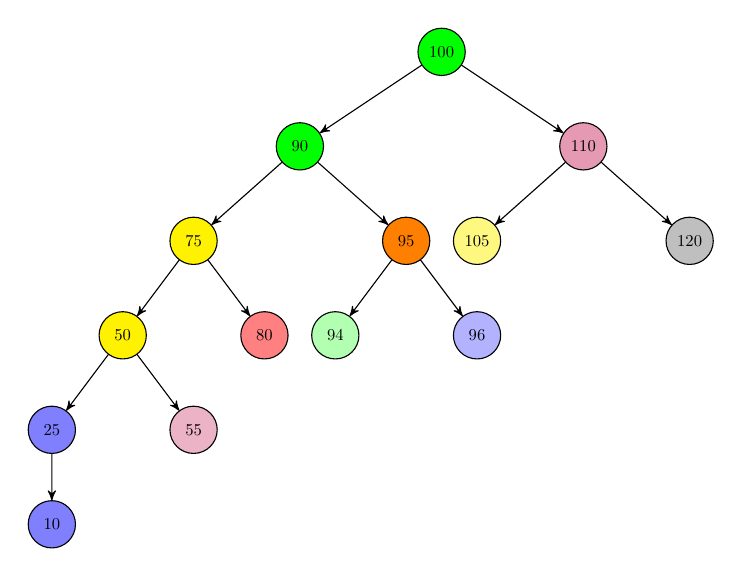
\begin{tikzpicture}[->,>=stealth',
					    level/.style={level distance = 2cm},
					    level 1/.style={sibling distance=6cm},
					    level 2/.style={sibling distance=4.5cm}, 
					    level 3/.style={sibling distance=3cm}, 
					    scale=0.6, transform shape]
            		\node [tr, fill=green] {100}
            		child {
            			node [tr, fill=green] {90} 
            			child {
            				node [tr, fill=yellow] {75} 
            				child {
            					node [tr, fill=yellow] {50} 
            					child{
            						node [tr, fill=blue!50] {25}
            						child{
            							node [tr, fill=blue!50] {10}
            						}
            					}
            					child{
            						node [tr, fill=purple!30] {55}
            					}
            				}
            				child {
            					node [tr, fill=red!50] {80} 
            				}
            			}
            			child {
            				node [tr, fill=orange] {95}
            				child{
            					node [tr, fill=green!30] {94}
            				}
            				child{
            					node [tr, fill=blue!30] {96}
            				}
            			}
            		}
            		child {
            			node [tr, fill=purple!40] {110}
            			child{
            				node [tr, fill=yellow!50] {105}
            			}
            			child{
            				node [tr, fill=gray!50] {120}
            			}
            		}
            		;
            		\end{tikzpicture}
            	}
            \end{figure}
            
            
            
            
            Het valt op dat wanneer we een niveau zeepbellen toevoegen, we het dubbele aantal toppen moeten toevoegen van de vorige zeepbelboom met een niveau lager. 
            Voor $n$ het aantal toppen en $z$ het aantal niveaus in zeepbellen geldt: $$n \ge \sum\limits_{i=1}^z k2^{z-1} = k(2^z-1)$$ 
            We lossen dit op naar $z$: $$z \le \log_2{(\dfrac{n+k}{k})}$$
            De maximale diepte $d_t$ van deze zeepbelboom in toppen is gelijk aan het aantal niveaus zeepbellen vermenigvuldigd met het maximale aantal toppen per zeepbel.
            Dus krijgen we dat $d_t=k\cdot z$.
            Wanneer voegen dit alles samen tot één formule:
            $$d_t \le k \cdot \log_2{(\dfrac{n+k}{k})}$$
            Waar $d_t$ gelijk is aan de maximale diepte in toppen.
    \endgroup 
\end{enumerate}
    \end{opgave}	
    \begin{opgave}
        Analyse van de verschillende gebalanceerde zeepbelbomen en hun complexiteit.
        \begin{enumerate}[a.]
            \item Voor toevoegen.

                \normalfont
                Het toevoegen van een item aan een gebalanceerde zeepbelboom gebeurt als volgt:

                Eerst wordt het item opgezocht in de zeepbelboom.
                Wanneer het item gevonden werd dan zit het item al in de zeepbelboom en moet er niets gebeuren.
                In dit geval heeft deze bewerking dezelfde tijds- en geheugencomplexiteit als het opzoeken, nl. $\mathcal{O}(\log n)$ (dit bespreek ik in punt $b$).
            \item Voor opzoeken.
                
                \normalfont
                De drie gebalanceerde zeepbelbomen gebruiken alledrie dezelfde opzoekmethode, dus de complexiteit van deze bewerking is dezelfde.
                Deze methode werkt zoals een normale binaire zoekboom: 
                
                De wortel wordt vergeleken met het gezochte item. Is het item in de wortel kleiner dan dalen we af naar het rechterkind van de wortel. 
                Is het item in de wortel groter dan dalen we af naar het linkerkind van de wortel.
                Komt de waarde van de wortel overeen met dat van het gezochte item dan hebben we het item gevonden en kunnen we terugkeren uit de functie.
                We blijven op deze manier zoeken tot we het gezochte item gevonden hebben of tot we niet meer verder kunnnen afdalen in de zoekboom (als we null tegenkomen).
                In dit geval zit het gezochte item niet in de zeepbelboom.

                \begin{enumerate}
                    \item Tijdscomplexiteit

                In het slechtste geval zit het item dat wordt gezocht niet in de zeepbelboom en moeten we helemaal tot een blad van de boom afdalen.
                In de vorige opgave heb ik beweze dat de maximale diepte (in toppen) gelijk is aan $d_t \le k \cdot \log_2{(\dfrac{n+k}{k})}$.
                $k$ is hier een constante, dus in asymptotische notatie valt deze weg.
                We komen dus uit dat het opzoeken van een element in een gebalanceerde zeepbelboom die $n$ items bevat een tijdscomplexiteit van $\mathcal{O}(\log n)$ heeft.
            \item Geheugencomplexiteit

                De implementatie van de zoekbewerking maakt gebruik van de {\tt find()} methode. Deze maakt gebruik van een {\tt while}-loop om in de boom af te dalen en maakt geen gebruik van andere datastructuren.
                De geheugencomplexiteit om iets op te zoeken in een gebalanceerde binaire boom is dus $\Theta(1)$.
        \end{enumerate}
        \end{enumerate}
    \end{opgave}



    \part*{Implementatie}
    Hieronder volgt er een korte uitleg over de interne structuur en algoritmes die
    ik heb gebruikt voor de implementaties van de zeepbelbomen.
    \section{Binaire boom}
    \subsection{Top}
    Mijn binaire boom bestaat intern uit toppen die hun ouder,  linker en
    rechterkind bijhouden. Om problemen met deze links te vermijden kan de verwijzing
    naar de ouder van een top enkel ingesteld worden wanneer deze top als kind wordt
    aangeduid van een andere top met de methodes {\tt setRightChild()} en {\tt setLeftChild()}. Omdat de wortel van de binaire boom natuurlijk geen
    ouder heeft is er ook een methode die deze verwijzing op {\tt null} zet.
    Een top bevat ook een booleaanse waarde {\tt removed} die functioneert als
    grafsteen. Daarnaast bevat iedere top ook een verwijzing naar de zeepbel waartoe die 
    top behoort.
    \subsection{Zeepbel}
    Om de toppen in groepjes in te delen bestaat de klasse {\tt Zeepbel}. Deze houdt
    enkel zijn wortel bij en het aantal toppen dat deze bezit. Een zeepbel heeft ook de
    methodes {\tt topAdded()} en {\tt topsRemoved()} die de zeepbel waarschuwen wanneer
    er toppen bijgekomen of weggevallen zijn. De methode {\tt topAdded()} heeft ook
    een boolean terug die zegt of de zeepbel te groot is en verkleind moet worden.
    \subsection{Zeepbelboom}
    In de abstracte klasse Zeepbelboom zit de gemeenschappelijke functionaliteit die
    alle zeepbelboom-implementaties delen. Het is enkel de methode {\tt shrinkBubble()}
    die verschilt tussen de verschillende zeepbelbomen. Deze methode zorgt ervoor dat een 
    overvolle zeepbel gesplitst wordt.

    \section{Implementaties zeepbelboom}
    \subsection{Zeepbelboom1}
    De eerste zeepbelboom  lost een overvolle zeepbel op door zo weinig mogelijk
    veranderingen te brengen aan de interne structuur van de boom. Wanneer de wortel van
    de overvolle zeepbel beide kinderen in diezelfde zeepbel heeft dan worden er geen
    wijzigingen aangepast aan de interne structuur: deze twee kinderen vormen de wortels
    voor twee nieuwe zeepbellen en de top wordt toegevoegd aan de bovenliggende zeepbel.
    Als de wortel van de zeepbel maar één kind in dezelfde zeepbel bevat worden de
    eerste drie toppen geroteerd zodat de wortel wel twee kinderen in dezelfde zeepbel
    heeft en er kan gesplitst worden zoals normaal.
    \subsection{BalancingBubbleTree}
    Dit is een superklasse voor alle zeepbelbomen die een zeepbel moeten kunnen balanceren.
    Deze balancering gebeurt door de methode {\tt balanceBubble()}. Dit gebeurt door eerst 
    alle toppen in inorde te overlopen en in een lijst te plaatsen.
    Vervolgens wordt van deze lijst een nieuwe binaire boom opgebouwd door de recursieve
    methode {\tt listToTree()}. Dit balanceren gebeurt in $\Theta (n)$ tijd als we het
    aantal te balanceren toppen als $n$ kiezen. Maar er wordt enkel in één zeepbel
    gebalanceerd en een zeepbel heeft een maximaal aantal toppen, dus werkt deze methode
    in constante tijd.   
    \subsection{Zeepbelboom2}
    Voor de zeepbel gesplitst wordt wordt deze eerst gebalanceerd met de methode
    uit {\tt BalancingBubbleTree}. Daarna wordt op dezelfde manier gesplitst als
    {\tt Zeepbelboom1}.
    \subsection{Zeepbelboom3}
    Deze zeepbel werkt op dezelfde manier als {\tt Zeepbelboom2} echter worden er hier
    zoveel mogelijk toppen aan de bovenliggende zeepbel toegevoegd. Deze zeepbelboom
    kan geconfigureerd worden: er kan gekozen worden om een maximum te zetten op het 
    aantal omhoog te duwen toppen en er kan ingesteld worden dat er geprobeerd wordt
    om net genoeg toppen toe te voegen aan de bovenliggende zeepbel dat die verplicht
    wordt om te splitsen.  
    \section{Functies}
    \subsection{Iterator}
    Een top heeft een methode {\tt traverseInorder()} waarmee er in inorde kan
    geïtereerd worden over zijn kinderen. Aan deze methode worden twee functionele
    interfaces meegegeven: een {\tt consumer} waaraan het volgende element in de iteratie
    wordt aan doorgegeven en een {\tt predicate} die extra restricties kan opleggen over
    welke toppen er geïtereerd mag worden (bijvoorbeeld enkel over de toppen van een
    bepaalde zeepbel.
    Alle iterators maken van deze methode gebruik.
    \subsection{\tt Zeepbelboom.find()}
    De drie basisoperaties: {\tt add()}, {\tt contains()} en {\tt remove()} maken gebruik
    van de methode {\tt find()} om een top op te zoeken. Deze methode werkt door binair
    te zoeken naar een {\tt Top} tot de juiste top gevonden is of tot er {\tt null} werd
    gevonden, waarna de top aan de juiste consumer wordt doorgegeven.
    \subsection{\tt Zeepbelboom.add()}
    Er wordt eerst met {\tt find()} gezocht naar de juiste top, als de top werd gevonden
    dan gebeurt er niets en wordt {\tt false} teruggegeven. Als de top niet werd gevonden
    wordt top toegevoegd op de plaats waar {\tt null} werd tegengekomen en wordt de
    betreffende zeepbel verwittigd van deze toevoeging, waarna er eventueel kan gesplitst
    worden als deze zeepbel overvol is.
    \subsection{\tt Zeepbelboom.contains()}
    Hier wordt enkel met {\tt find()} gezocht en teruggegeven of de top gevonden werd
    of niet.
    \subsection{\tt Zeepbelboom.remove()}
    De te verwijderen top wordt opnieuw gezocht met {\tt find()}. Wanneer de top gevonden
    werd wordt er een grafsteen geplaatst door de {\tt removed} waarde op {\tt true} te
    zetten. Als er een kritiek aantal grafstenen wordt bereikt (standaard 50\%) wordt
    de boom opnieuw opgebouwd zonder de grafstenen.
    \newline \newline
    Ik was begonnen met een implentatie die de toppen echt uit de zeepbelboom verwijdert,
    maar helaas zitten er nog wat bugs in de code en had ik geen tijd meer om deze te
    debuggen. Dus heb ik een werkende implementatie met grafstenen gemaakt.

    
    
    \newpage
    \part*{Experimenten}
    Nu volgen de resultaten van enkele testen die ik heb uitgevoerd op de zeepbelbomen.
    \end{document}
